\chapter{混部场景导向的调度定制}\label{chap:sched_policy}

% Core调度框架定制(静态) -> BPF任务调度机制定制(动态) -> 资源感知调度机制定制(动态) -> 资源感知调度策略定制(动态) 

为解决不同混部场景下任务调度机制的不足,本章主要展开混部场景导向的定制任务调度机制研究。首先,从内核任务调度的相关配置上,针对不同应用的需求,设计了响应度优先与吞吐量优先两种基础内核配置,随后,在Ext调度类的基础上研究场景导向的BPF Scheduler定制,设计了基于调度队列隔离的QoS保障策略,并在此基础上,结合eBPF的监测能力,进一步设计了CPU资源感知与网络资源感知的任务调度策略。

\section{内核调度配置定制}

Linux调度子系统提供了一些编译配置选项,用以针对场景进行优化,相关配置选项围绕时钟中断与抢占模型展开。

时钟中断是驱动Linux抢占式调度的核心机制,如表~\ref{tab:config_hz}所示,Linux内核提供了时钟中断频率与时钟中断处理模式两方面的配置。其中,中断的频率配置决定了调度滴答的周期,Linux提供了从100、250、300到1000四种不同的中断频率配置,一方面,越高的时钟中断频率意味着系统的整体响应度更好,另一方面,时钟中断频率决定了时间片的最小粒度,Linux在每个时钟中断中处理时间片记账,然而时钟中断间隔中存在任务切换的可能,容易导致时间记账的误差,而越高的时钟中断频率意味着越小的时钟中断间隔,间隔中发生任务切换的概率也会越小,因此越高的时钟中断频率意味着更准确的时间记账。

\begin{table}[H]
    \bicaption{\quad 内核时钟中断配置}{\quad Kernel Clock Interrupt Configuration}% caption
    \label{tab:config_hz}
    \footnotesize% fontsize
    \setlength{\tabcolsep}{4pt}% column separation
    \renewcommand{\arraystretch}{1.25}% row space 
    \centering
    \begin{tabular}{lc}
        \hline
        配置名称 & 描述 \\
        \hline
        HZ\_100  & 配置时钟中断频率为100  \\
        HZ\_250  & 配置时钟中断频率为250 \\
        HZ\_300  & 配置时钟中断频率为300 \\
        HZ\_1000 & 配置时钟中断频率为1000 \\
        HZ\_PERIODIC & 永远不要忽略时钟中断 \\
        NO\_HZ\_IDLE & 忽略空闲CPU上的时钟中断 \\
        NO\_HZ\_FULL & 忽略空闲CPU,以及只有一个可运行任务CPU上的时钟中断 \\
        \hline
    \end{tabular}
\end{table}

时钟中断会打断当前任务的执行,并产生上下文切换的开销,为此Linux内核提供了如表~\ref{tab:config_hz}所示的不同时钟中断处理模式,来减少特定场景中的不必要的时钟中断开销。在开启NO\_HZ选项之后,Linux内核允许指定部分CPU核心为NO\_HZ核心,而根据不同的时钟处理模式,这些CPU会在特定的场景下,如CPU空闲时,忽略时钟中断,以达到节能或减少对任务的干扰的目的。

抢占通常指高优先级任务打断低优先级任务的执行。在Linux内核中,中断产生时用户态任务总是会被抢占,但对于内核态代码,早期Linux内核在执行时会屏蔽中断,而在一些较长的内核代码处理路径中就容易导致系统整体的响应度下降。为此内核提供了如表~\ref{tab:config_preempt}所示的抢占模型,用于定制内核代码执行对于中断的处理模式,不同抢占模式的主要区别在于内核代码可被抢占位点的差异,而内核代码中可被抢占的位点越多,系统的实时性就会越好,但也同时也意味着任务的执行更容易被频繁地打断,因此需要根据不同应用的需要来进行选择。

\begin{table}
    \bicaption{\quad 内核抢占模式配置}{\quad Kernel Preemption Configuration}% caption
    \label{tab:config_preempt}
    \footnotesize% fontsize
    \setlength{\tabcolsep}{4pt}% column separation
    \renewcommand{\arraystretch}{1.25}% row space 
    \centering
    \begin{tabular}{lc}
        \hline
        配置名称 & 描述 \\
        \hline
        PREEMPT\_NONE  & 内核代码保持执行直到主动放弃CPU  \\
        PREEMPT\_VOLUNTARY  & 开启了内核代码中的抢占位点 \\
        PREEMPT  & 提供更多的内核代码抢占位点,实现完全抢占 \\
        PREEMPT\_RT & 进一步修改内核代码的实现,如锁机制,实现实时可抢占性 \\
        \hline
    \end{tabular}
\end{table}

时钟中断和抢占模式配置共同决定了Linux调度子系统的整体响应度,根据应用的不同需求,本研究设计了响应度优先与吞吐量优先两种基本调度子系统内核配置。其中,响应度优先配置采用更高的HZ与激进的抢占模式来提升整体响应度,满足应用对于延迟与实时性的需求。吞吐量优先配置则采用较低的HZ与保守的抢占模式,让CPU在有限的时间内更多的执行任务而不是中断处理,来满足应用对于局部性和性能的需求。

\section{BPF任务调度机制设计}

% 混部Linux优先级机制的问题
% - 调度队列优先级问题: 
%  - 优先级机制用于限制不同任务对CPU时间的使用,并不能保证高优先级的应用一定能够比低优先级应用优先调度
% - 调度类优先级问题:
%  - 运行在实时调度类中的LC任务如配置不当,一方面不利于应用性能,另一方面容易造成系统崩溃
%  - 将低优先级的任务允许在Idle类是嵌入式领域的常用做法,但不够灵活,且违背Linux设计语义
% 解决方式
% - 引入Ext调度类,使能调度队列隔离
% - 利用BPF Scheduler的灵活性
% 调度器架构
% - User Input: Task define, Resource define
% - eBPF Input: Task status, Resource status
% - Control Signals: BPF Map、BPF Prog: rodata\bss
% - BPF Scheduler: Select Eligible Task to Eligible CPU
% - Control: BPF Helper \ User Define Command \ eBPF Define
% 调度模式
%  - 全局调度
%  - Per-CPU调度
% 调度策略
%  - FIFO
%  - RR
%  - Vtime

混部场景中使用优先级机制来保障高优先应用QoS是常用的手段,Linux提供了调度类与调度队列两层的优先级定义,然而在应用的QoS上保障上两层优先级的机制都存在一定的不足。

在调度类层,利用调度类的优先级差异能够保证高优先就绪时总是能够抢占低优先应用,从而实现高优先应用的QoS保障。优先级差异可以通过将高优先应用添加到较高优先级的调度类,或者将低优先应用添加到低优先级调度类实现。将高优先应用添加到高优先级调度类时,需要充分考虑应用的特点与高优先级调度类的配置,不恰当的配置一方面会影响应用本身的性能,另一方面也有可能引发整个系统性能下降。将低优先任务添加到低优先级调度类,如Idle调度类时也存在风险。首先,将常规任务放置到Idle调度类破坏了Idle调度类的设计语义,不利于系统能耗。其次,Idle调度机制十分基础,无法满足不同低优先任务的调度需求。

在调度队列层,以默认的CFS调度为例,CFS提供从-20到20的静态优先级,能够影响应用vruntime的积累速度。高优先应用的vruntime相对增加得缓慢,通常能够得到更多的调度机会,但是随高优先应用的vruntime不断累积,在CFS公平调度的机制实现下,存在在被低优先应用抢占的可能。同时,CFS调度器中包含了许多不利于高优先应用QoS保障的启发式逻辑。CFS的执行过程中会为每个调度队列维护一个基准的vruntime,通常是调度队列中vruntime的最小值,新创建和刚唤醒的进程会被赋予基准vruntime值,并在CFS调度算法下得到优先执行。然而,这一启发式逻辑没有考虑到进程之间的优先级,当低优先级大量唤醒或创建时,高优先应用反而会被频繁抢占并产生QoS劣化。其次,调度队列层优先级无法跨CPU地产生作用,这一方面导致高优先应用与运行在其他CPU上的低优先应用争抢资源,另一方面使得高优先应用在不同CPU上迁移时相对优先级变化而导致优先性丧失。

为解决混部场景下Linux任务调度在QoS保障上的问题,本研究设计了基于Sched Ext项目的BPF任务调度机制,能够在保障高优先任务全局优先性的同时支持灵活的调度策略。首先,Ext调度类处于Fair调度类与Idle调度类之间,将低优先任务添加到Ext调度类中可构建调度类优先级差异,从而实现高优先应用就绪时总是能够抢占低优先应用。同时,由于调度类优先级是系统全局的,因此能够在各个CPU以及跨机器迁移时生效。其次,针对不同混部场景下应用的不同需求,BPF任务调度机制能够针对性地进行设计,从而根据实际情况更好地进行高优先任务的QoS保障。

BPF任务调度机制架构如图~\ref{}所示,框架的核心是BPF调度器,基于Ext提供的接口实现,能够定制Ext调度类的任务调度行为。除此之外,本研究向BPF调度器引入了额外的数据输入源,包括用户与其他子系统的数据输入。额外的输入数据通过BPF Map等机制提供给BPF调度器,用以辅助进行调度决策。同时BPF调度器也能够通过共享内存的方式将数据提供给用户态程序,并借助与用户态程序的协作实现更灵活的任务调度。

% TODO: 总体架构图

BPF任务调度机制支持用户与eBPF外部数据源,区别于Ext调度类提供的调度信息,外部数据源的信息可以由用户自定义或从其他子系统中采集。其中,用户数据源作用在BPF调度器初始化和运行时。一方面,用户可定义CPU资源拓扑、BPF调度器参数等,并在在BPF初始化时通过修改BPF程序的rodata、bss段来将静态信息传递给BPF调度器。另一方面,BPF调度器通过预先声明BPF Pin Map来向外部暴漏数据入口,用户程序则可以通过读写BPF Pin Map来与BPF调度器交互,如传递用户对于进程、Cgroup的优先性、类型、资源需求的声明。eBPF外部数据源则通过在其他子系统中插桩,如内核资源分配的关键路径、系统调用等,获取其他子系统的运行状态,这些信息可以直接通过BPF Map共享给BPF调度器,同时,eBPF插桩也可根据混部场景的需要自由选择与定制。

BPF调度器既可以直接定制Ext调度行为,也可以在调度过程中利用上述的额外数据源来针对性地调整调度行为,同时,BPF调度器也可以通过BPF Map来将调度信息共享给用户程序与其他子系统,并利用用户程序的灵活性以及eBPF在其他子系统如网络子系统上的定制能力。同时,BPF任务调度机制还提供了可选的基本调度机制和调度策略。

% TODO: 调度模式图 a \ b

在调度模式上,BPF任务调度机制支持Per-CPU调度与全局调度两种调度模式。Per-CPU调度是Linux中常用的调度模式,通过将调度卸载到各个CPU上来避免共享内存导致的竞争,BPF调度框架中通过为每个CPU创建一个BPF DSQ,并将调度策略限制在本地CPU的BPF DSQ上来实现Per-CPU调度。Per-CPU调度模式适用于CPU数量较多且对调度开销要求较高的场景。在延时敏感的混部场景中,将调度延时降低到应用的延时阈值内是保障QoS的一种方式,受限于内核的HZ配置,Per-CPU调度延时最小为1ms(1000HZ),同时,由于Linux HZ配置是全局的,而较高的时钟中断会导致整个系统中时钟中断处理的资源使用增大,影响CPU敏感任务的执行。而为解决调度延时的问题,BPF任务调度机制提供了全局调度模式。全局调度模式基于全局调度队列与高精度时钟实现,与其他研究类似,首先选择一个CPU作为调度核心,并在这个CPU上创建全局的DSQ。同时,在调度核心上设置一个BPF Timer,利用高精度时钟实现ns级的调度周期。全局调度模式的调度过程中,首先将新创建的任务加入到全局DSQ上,每次BPF Timer的回调中,调度核心会更新任务的记账信息并尝试调度任务,并抢占时间片耗尽的任务,其中调度核心与其他核心的交互通过IPI实现。

在调度策略上,为适应不同混部应用的调度需求,BPF调度框架提供了三种基本的调度策略实现:

\begin{enumerate}
    \item \textbf{基于FIFO的非抢占式调度}:BPF调度器中使用FIFO DSQ(分发队列),并设置每个入队任务的时间片为无限,任务运行直到主动退出,随后BPF调度器取出下一个任务执行。
    \item \textbf{基于RR的抢占式调度}:BPF调度器中使用FIFO DSQ, 并按照配置设置每个入队任务的时间片,每次时钟滴答时检查当前任务的剩余时间片,抢占时间片耗尽的任务并切换到下一个任务执行。
    \item \textbf{基于vtime的抢占式调度}:BPF调度器中使用vtime DSQ,vtime DSQ按照vtime大小对任务进行排序,初始时设置每个入队任务的初始vtime,并在每个时钟滴答里根据任务的静态优先级更新vtime,并进行抢占判断。当抢占发生时,vtime越小的任务越优先被调度。
\end{enumerate}

相较于Linux任务调度机制,BPF任务调度机制能够提供更灵活的任务调度机制与调控手段,并通过定制和组合不同的外部数据来源、调度模式与调度策略来满足不同混部场景应用对调度机制的需求,从而更好地保障高优先应用的QoS。

\section{资源感知的BPF任务调度}

% 对于CPU资源的隔离,常见的方式是显示地隔离不同应用能够使用的CPU,这种静态的划分方式并不能有效的使用资源,而在本章中提出了基于BPF调度器的调度队列隔离,高低优先级的应用在调度队列优先级机制之上共享相同CPU,使得高优先级应用运行时总是能够优先地使用CPU资源。

% 其次,相较于常见的调度类隔离,本章基于BPF调度器实现更为灵活,通过结合eBPF强大的监测能力,让BPF调度器感知高优先级应用CPU资源、网络资源的使用,而通过设置相关的资源约束,从而结合不同高优先级应用的资源使用特征与调度目标,更充分的利用资源。

\subsection{CPU资源感知的任务调度} 

% 进行CPU资源隔离的原因
% CPU Set静态资源划分的问题
% CPU资源感知机制的实现
% - 用户定义的CPU拓扑
% - Ext调度类eBPF hook
% CPU资源感知策略的实现
% - 保守调度场景
% - SMT场景 

CPU拓扑描述了CPU之间的资源共享情况,而CPU之间的资源共享是混部场景中“吵闹邻居”的核心原因。调度时需要考虑CPU间的拓扑关系,而使用CPU Affinity机制将不同应用划分到不同的CPU集合中是常用方式,然而这种方式存在一些缺陷。首先,CPU Affinity隔离粒度较粗,划分不当容易造成CPU资源浪费。其次,静态的CPU集合划分没有考虑到应用CPU资源使用的动态特性,较保守的策略容易造成资源浪费,而激进的策略则容易引发QoS劣化。

造成上述问题的核心在于划分CPU集合时并没有考虑到不同应用对CPU资源的实际使用情况,而为解决这一问题,本研究设计了CPU资源感知的任务调度策略,调度逻辑如伪代码~\ref{alg:cpu_aware_sched}所示,通过增加外部数据源的方式,让低优先任务感知高优先应用使用CPU资源的情况,并结合用户输入的CPU拓扑判断是否需要出让CPU资源,从而实现高优先应用的QoS保障。

\begin{algorithm}
    \caption{Pseudocode for Enhanced Task Scheduling Isolation Mechanism}
    \label{alg:cpu_aware_sched}
    \begin{algorithmic}[1]
    
    \Function{cpuAcquire} {cpu}
    \State Insert cpu to CPU\_Map;
    \EndFunction
    
    \Function{cpuRelease} {cpu}
    \State Remove cpu from CPU\_Map;
    \EndFunction
    
    \Function {schedule}{}
        \While{True}
            \If{$\text{CPU\_Acquired + CPU\_Idle} < \text{CPU\_Available}$ }
                \State Set Exclusive Flag;
                \For{each no\_hz core C}
                    \State Send an IPI to envoke target CPU rescheduling.
                \EndFor
                \State Yield to higher priority scheduler class;
            \EndIf
            \State Remove Exclusive Flag;
            \State Dispatched tasks;
        \EndWhile
    \EndFunction
    \end{algorithmic}
\end{algorithm}

CPU资源感知的任务调度策略基于BPF任务调度机制实现。首先,在BPF程序初始化时,用户需要传入当前系统CPU拓扑以及低优先任务所能使用的CPU数量。随后,BPF程序初始化过程中会创建一个全局数组记录Ext调度类所管理的CPU状态,并通过在Ext调度类cpu\_acquire与cpu\_release处的插桩动态更新。任务调度时,BPF调度器读取全局数组,计算得到当前低优先任务能够使用的CPU数量,并与阈值进行比较。当不满足CPU阈值时,拒绝进行任务调度,而目标CPU会在Local DSQ没有任务执行时,出让CPU并被Idle调度类抢占。而当CPU满足阈值时,BPF调度器首先将任务调度到目标CPU的Local DSQ上,并根据目标CPU的状态来决定是否需要发送IPI。

BPF任务调度机制提供了以调度队列为粒度的CPU资源划分,相较于CPU Affinity粒度更细。借助调度类优先级差异,低优先任务能够在高优先任务运行时及时出让CPU资源,从而实现动态的CPU资源分配。然而这种资源的出让没有考虑CPU的拓扑关系,在如SMT作为底层硬件的混部场景中,无法有效地保障高优先应用的QoS。而CPU资源感知任务调度策略通过用户输入以及CPU资源的eBPF探测弥补了这一缺陷,能够更好地在SMT以及激进的高优先任务QoS保障场景中发挥作用。

\subsection{网络资源感知的任务调度}

% 网络资源感知的目标
% - 现有问题
% 网络资源感知机制的实现
% - Epoll系统调用eBPF hook
% - LC应用划分
% 网络资源感知策略的实现
% - LC应用低负载,高负载,负载高时,基于Epoll的LC应用特征变化(CPU敏感),要求吞吐量
% - 交还eevdf, 动态时间片

混部场景中LC应用通常为网络服务应用,在画像分析中发现,网络服务应用的资源使用倾向与敏感度在不同负载下存在差异。在负载较低时,由于请求量少、处理时间快,因此对资源的需求不高,且受到干扰影响不明显。而在负载较高时,对资源的需求激增,同时干扰会导致处理请求的速度变慢,而待处理请求的积压会引发较大QoS劣化。

\begin{algorithm}[H]
    \caption{Pseudocode for Network Resource Constraints Scheduling Strategy}
    \label{alg:network_aware_sched}
    \begin{algorithmic}[1]

    \Function {do\_epoll\_wait\_return}{$nr\_event$}
        \State Write timestamp of current epoll wait;
        \State Write $nr\_event$ of current epoll wait;
        \State Update total event count;
        \State Update count of epoll wait;
    \EndFunction

    \Function {schedule}{}
        \While{True}
            \State Read epoll wait delta from bpf map;
            \If{$\text{EPOLL\_WAIT\_DELTA} < \text{EPOLL\_WAIT\_THRESHOLD}$ }
                \State Set Exclusive Flag;
                \For{each no\_hz core C}
                    \State Send an IPI to envoke a rescheduling;
                \EndFor
                \State Yield to higher priority scheduler class;
            \EndIf
            \State Remove Exclusive Flag;
            \State Dispatched tasks;
        \EndWhile
    \EndFunction
    \end{algorithmic}
\end{algorithm}

实际生产环境中,网络服务应用的负载更加具有波动性,然而,Linux任务调度机制并不考虑混部应用在不同负载对于调度需求,同时也缺乏有效的应用负载感知机制。为解决上述问题,本研究设计了网络资源感知的任务调度策略,调度逻辑如伪代码~\ref{alg:network_aware_sched}所示,通过eBPF插桩获取应用的实时负载,并从用户输入获取目标应用在不同负载下的调度需求,并针对性地实施不同的调度策略,在低负载下以系统吞吐为目标,而在高负载时以高优先应用的QoS保障为目标。

高性能网络应用使用epoll作为底层的网络机制。epoll允许进程同时监听多个连接,并在连接就绪时进行批量处理,相较于阻塞型网络系统调用,使用epoll能够在大量请求时减少频繁地阻塞唤醒过程,从而支持更高的并发量。epoll机制涉及到多个系统调用,而其中最为核心的是epoll\_wait系统调用,进程在注册等待事件之后,就能够通过epoll\_wait系统调用来获取当前的就绪事件,当存在就绪事件时,epoll\_wait系统调用会返回就绪的事件数量,而当没有事件就绪时,epoll\_wait仍然会阻塞进程。

网络资源的感知基于epoll\_wait系统调用的eBPF插桩实现。具体代码中,首先创建两个Per-CPU BPF Map,分别记录Per-CPU上epoll\_wait系统的频率与事件数量,同时在key的选择上,支持pid、Cgroup以及系统三种监测粒度。而在eBPF插桩位点上,选择do\_epoll\_wait内核函数的返回位点,此处不仅表示一次epoll\_wait系统调用的完成,也能够通读取返回值,获取此次epoll\_wait系统调用所得到的epoll事件数量。每次计数完毕后,都会更新此次计数的时间戳,结合计数与时间戳数据,就能够计算应用的负载量。

在一个4CPU、1024MB内存的虚拟机中截取Redis、Memcached、Nginx与Mysql四个常见网络服务型应用在一段时间内的负载与epoll时间计数。如图~\ref{fig:epoll_request}所示,对于三种应用而言epoll事件与负载量高度相关,而考虑epoll事件的统计发生在服务端,而请求数量的统计发生在客户端,因此两端序列在时间上存在一定的偏移,同时,对于没有使用epoll作为底层网络机制实现的Mysql,这种监测方式就不能反映应用的网络资源使用,需要依赖其他的手段。由此也反映出,在不同的混部场景下,需要有不同的监测手段。

% TODO: 图例显示不全修正,增加nginx与 MySql
\begin{figure}[!htbp]
    \centering
    \begin{subfigure}[b]{0.49\textwidth}
        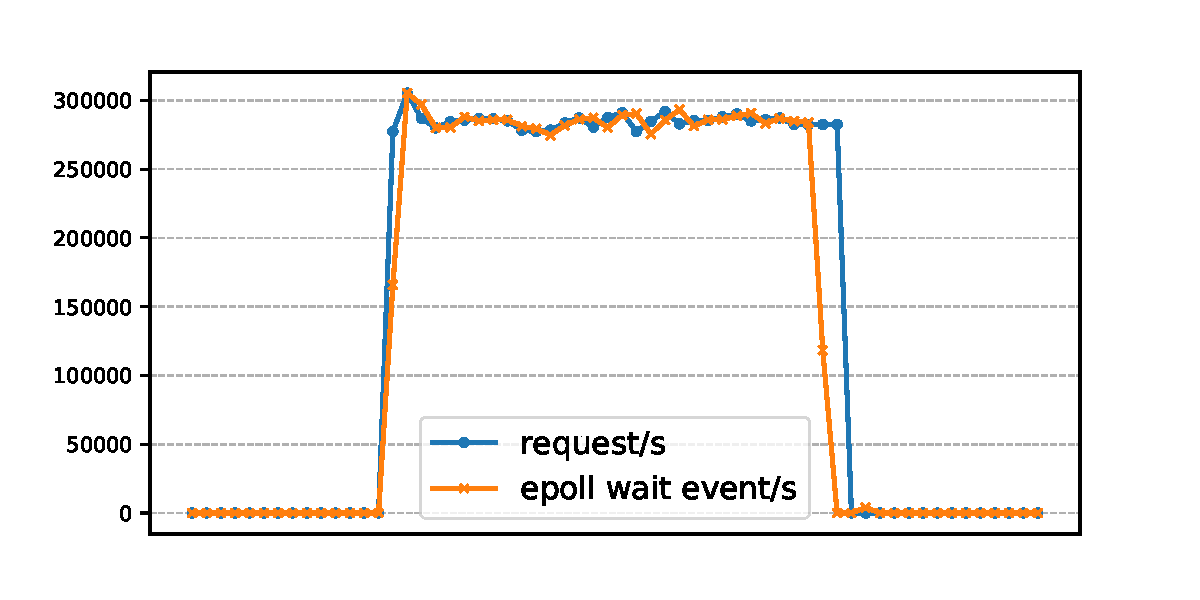
\includegraphics[width=\textwidth]{epoll_memcached}
        \caption{Memcached请求数量与Epoll Wait事件数量}
        \label{fig:epoll_memcached}
    \end{subfigure}
    \begin{subfigure}[b]{0.49\textwidth}
        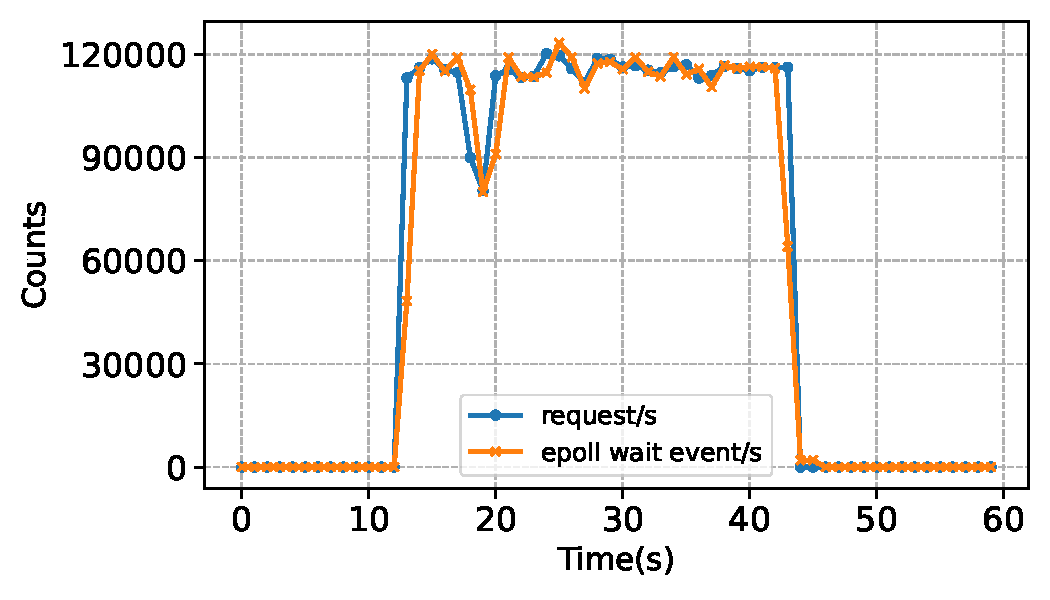
\includegraphics[width=\textwidth]{epoll_redis}
        \caption{Redis请求数量与Epoll Wait事件数量}
        \label{fig:epoll_redis}
    \end{subfigure}
    \begin{subfigure}[b]{0.49\textwidth}
        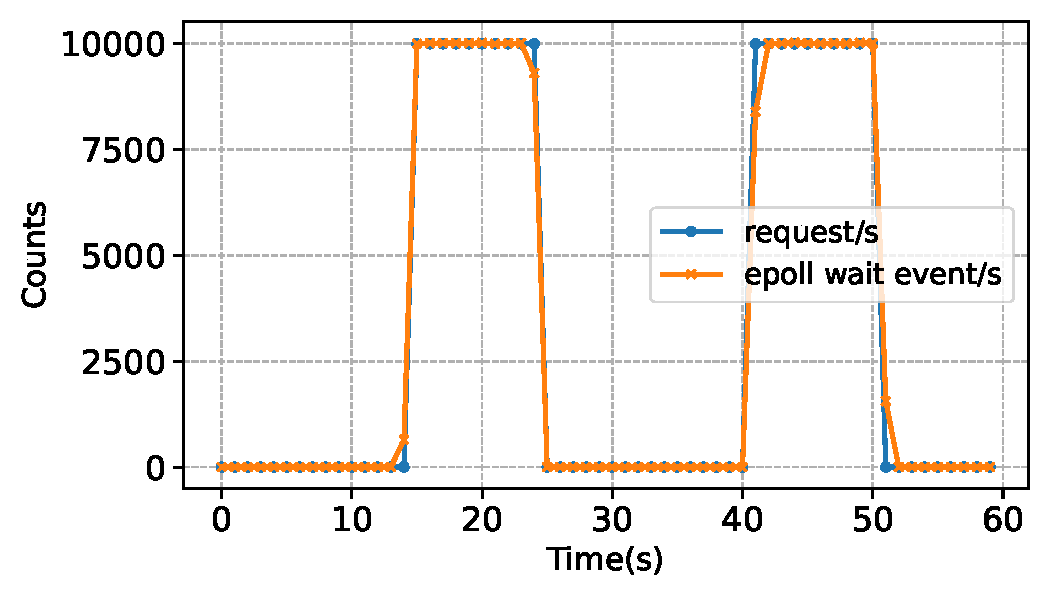
\includegraphics[width=\textwidth]{epoll_nginx}
        \caption{Nginx请求数量与Epoll Wait事件数量}
        \label{fig:epoll_nginx}
    \end{subfigure}
    \begin{subfigure}[b]{0.49\textwidth}
        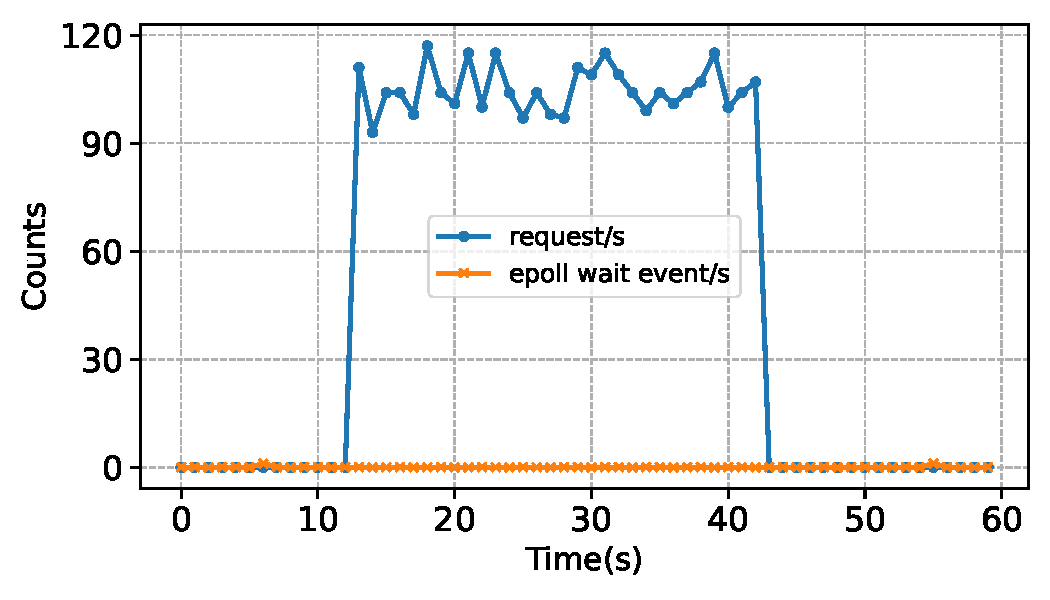
\includegraphics[width=\textwidth]{epoll_mysql}
        \caption{Mysql请求数量与Epoll Wait事件数量}
        \label{fig:epoll_mysql}
    \end{subfigure}
\bicaption{\quad LC应用负载与Epoll事件}{\quad Requests and Epoll Events on LC}
\label{fig:epoll_request}
\end{figure}

基于网络资源感知的任务调度机制实现也有多种实现的方式。首先,BPF调度器可以在调度时,参考高优先应用的负载情况,在低负载时,直接调度任务而不考虑CPU拓扑上的资源竞争,并调节时间片大小,在满足高优先低负载时的基本延时需求的同时,实现更高的系统吞吐。而在高负载时,采用避让的原则,减少与高优先应用的资源竞争,从而实现高优先应用的QoS保障。其次,也可以将探测逻辑与BPF调度器分离,如在低负载时,关闭BPF调度器,此时低优先任务会被Fair调度类调度,并与高优先应用处在相同的调度队列中,通过分时复用进一步提高吞吐,而在高负载时,加载CPU资源感知的BPF调度策略,并设置较为保守的参数来优先保障高优先应用的QoS。

% \subsection{基于PMU实现的其他资源感知策略}

\section{实验设计与分析}

\subsection{响应度优先内核性能}

% redis \ memcached

响应度优先任务调度配置使用HZ\_1000配置时钟中断频率,并配置PREEMPT抢占模式。实验在一个4CPU 1024MB内存的虚拟机上展开,并选择Redis、Memcached两种延迟敏感应用分别与干扰应用进行混部来构建混部场景,并与使用HZ\_250和VOLUNTARY抢占模式的CloudHypervisor默认Linux内核进行比较。

\begin{figure}[H]
    \centering
    \begin{subfigure}[b]{0.49\textwidth}
      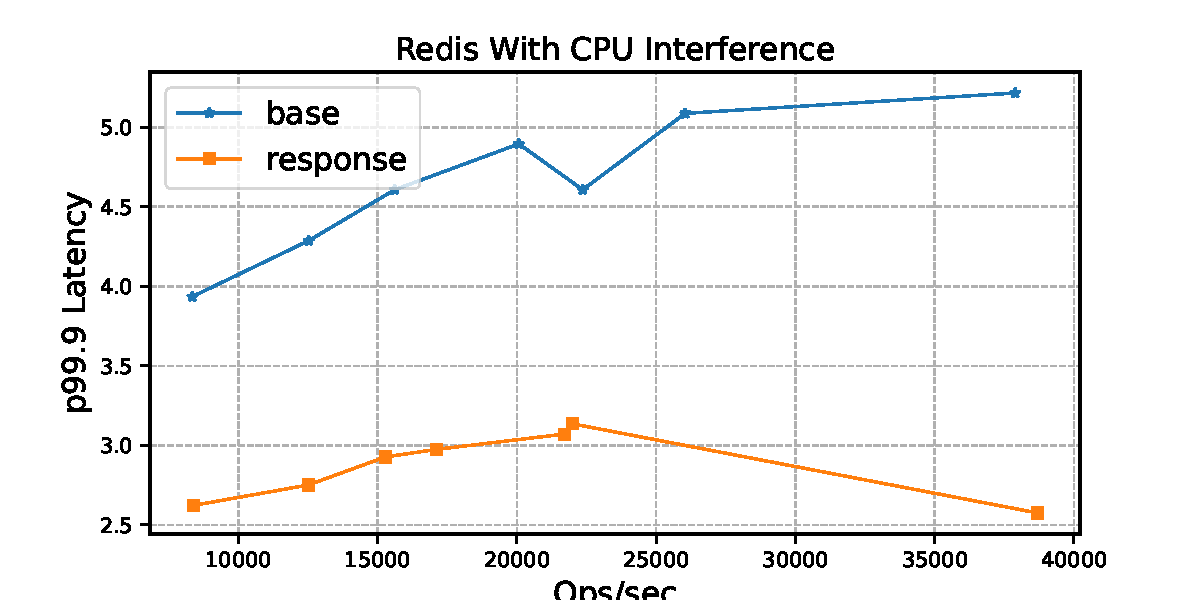
\includegraphics[width=\textwidth]{redis_response}
      \caption{Redis与干扰混部}
      \label{fig:redis_response}
    \end{subfigure}
    \begin{subfigure}[b]{0.49\textwidth}
      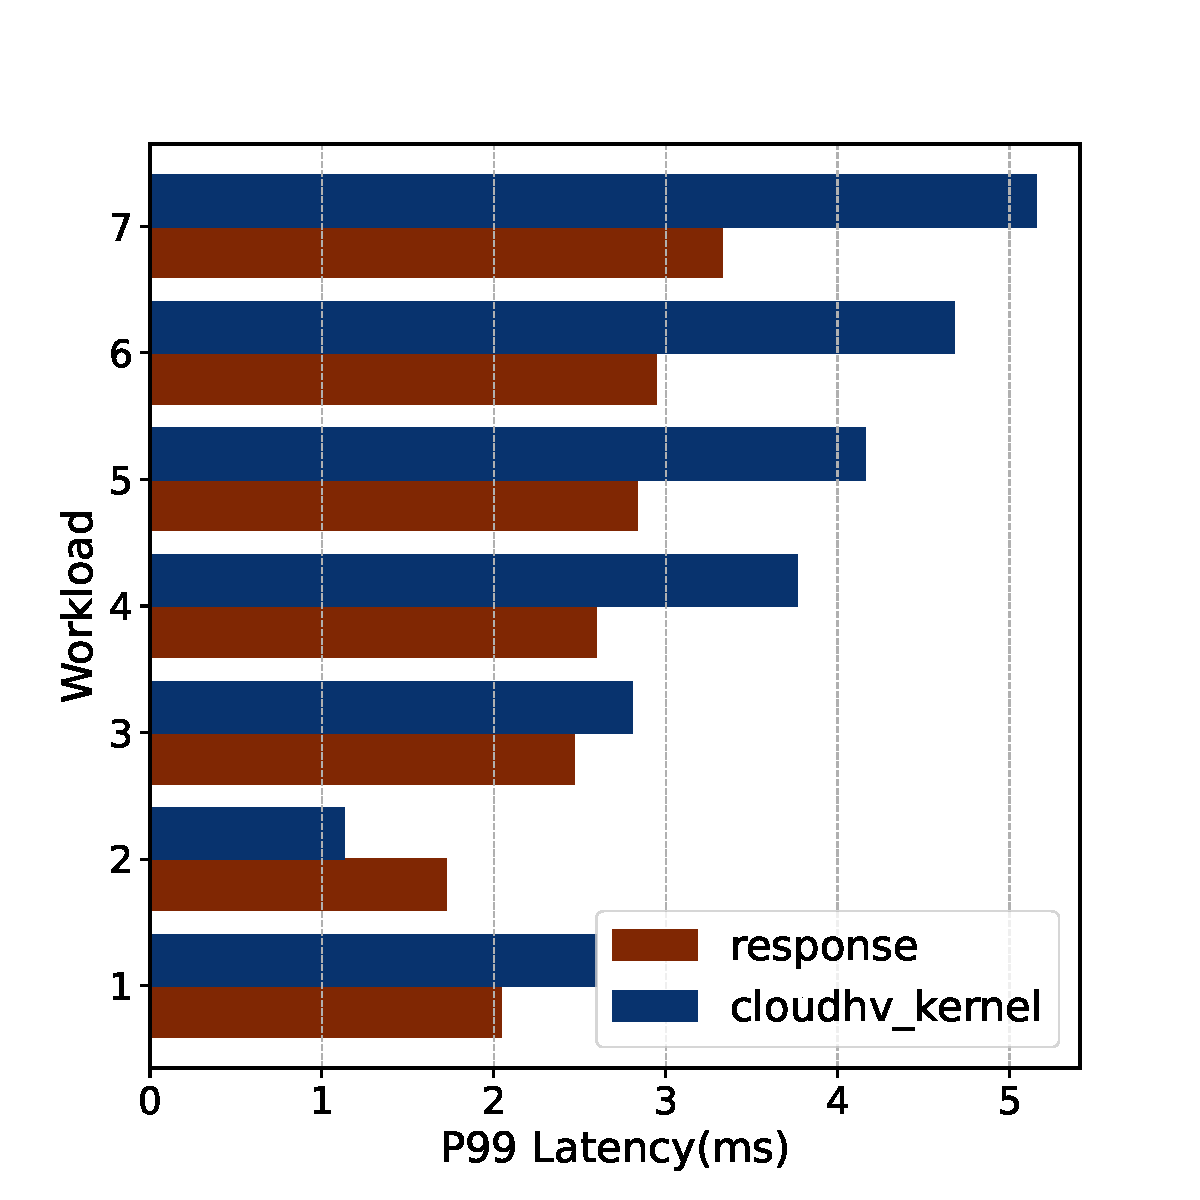
\includegraphics[width=\textwidth]{memcached_response}
      \caption{Memcached与干扰混部}
      \label{fig:memcached_response}
    \end{subfigure}
    \bicaption{\quad 混部场景下的响应度优先内核}{\quad Response Priority Kernel in Mixed Deployment Scenarios}
    \label{fig:lc_response}
\end{figure}

混部实验结果如图~\ref{fig:lc_response}所示,在启用Control Zone响应度优先内核后,无论是Redis还是Memcached,在P99.9延迟上都要优于CloudHypervisor的默认内核,Reponse内核使用了更高的时钟中断频率,因此能够更快地在延时敏感应用与干扰应用中进行切换,同时在PREEMPT抢占模式下,网络中断能够更及时地进行处理,降低请求处理链路的整体延时。

\subsection{吞吐量优先内核性能}

% graph500(time) \ ffmjpeg 

吞吐量优先任务调度配置使用HZ\_100配置时钟中断,并开启PREEMPT\_NONE抢占模式。实验在一个4CPU 1024MB内存的虚拟机上展开,并选择Graph500、ffmjepg两种CPU敏感型应用分别于干扰应用混部来构建混部场景,并与使用HZ\_250和VOLUNTARY抢占模式的CloudHypervisor默认Linux内核进行比较。

\begin{figure}[H]
    \centering
    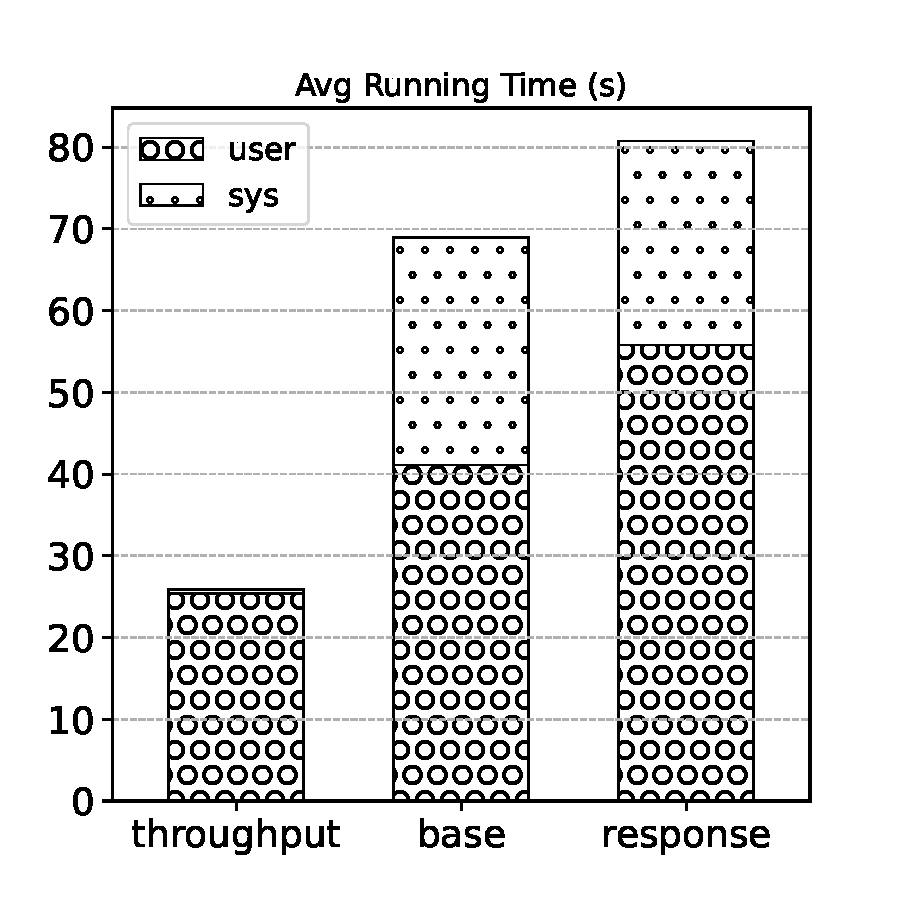
\includegraphics[width=0.5\textwidth]{avg_graph500_runtime}
    \bicaption{\quad 吞吐量优先内核配置优化效果}{\quad Throughput Discrepancy Across Different Configurations} 
    \label{fig:avg_graph500_runtime}
\end{figure}

Graph500主要执行图计算算法,因此执行时间是其重要的性能指标,实验中使用time工具记录任务的执行时间,包括用户态与内核态的执行时间, 具体实验结果如图~\ref{fig:avg_graph500_runtime}所示,其中使用Throughput内核的Control Zone消耗的时间最短,而使用Response内核的Control Zone则消耗的最长的时间,分析执行时间占比,在Throughput内核下,任务运行过程中内核态时间消耗几乎没有,而在Response内核中,内核态时间则占用了较大比例,造成这一结果的主要原因是时钟中断与NO\_HZ配置,越高的时钟中断频率会引发越导致越频繁的陷入内核态,一方面使得内核态时间变得更长,另一方面也会导致局部性的破坏导致任务执行速度的减慢。

\subsection{CPU资源感知策略效果}

% 普通场景
% 硬件场景:SMT

CPU感知BPF调度策略实验首先验证调度策略对高优先级任务的QoS保障能力,实验在一个4 CPU、1024MB内存的虚拟机中展开,其中高优先应用为Mysql与Memcached,低优先级应用为CPU干扰应用。混部结果如图~\ref{lc_bpf_sched}所示,总体来看,CPU资源感知策略能够使LC应用达到与未受干扰情况下相近的性能,如图~\ref{fig:bpf_sched_smp_mysql}所示,MySql性能最高提升了60.8\%,同时,如图~\ref{fig:bpf_sched_smp_memcached}所示,Memcached延迟最高降低了48.2\%,这一方面得益于Ext调度类在调度队列上的隔离性,使得高优先应用总是能够及时地得到调度,同时,通过CPU资源感知,进一步让其他核心上的低优先级任务感知高优先级任务的运行,并根据阈值来判断是否要出让CPU以避免干扰。

\begin{figure}[H]
    \centering
    \begin{subfigure}[b]{0.49\textwidth}
        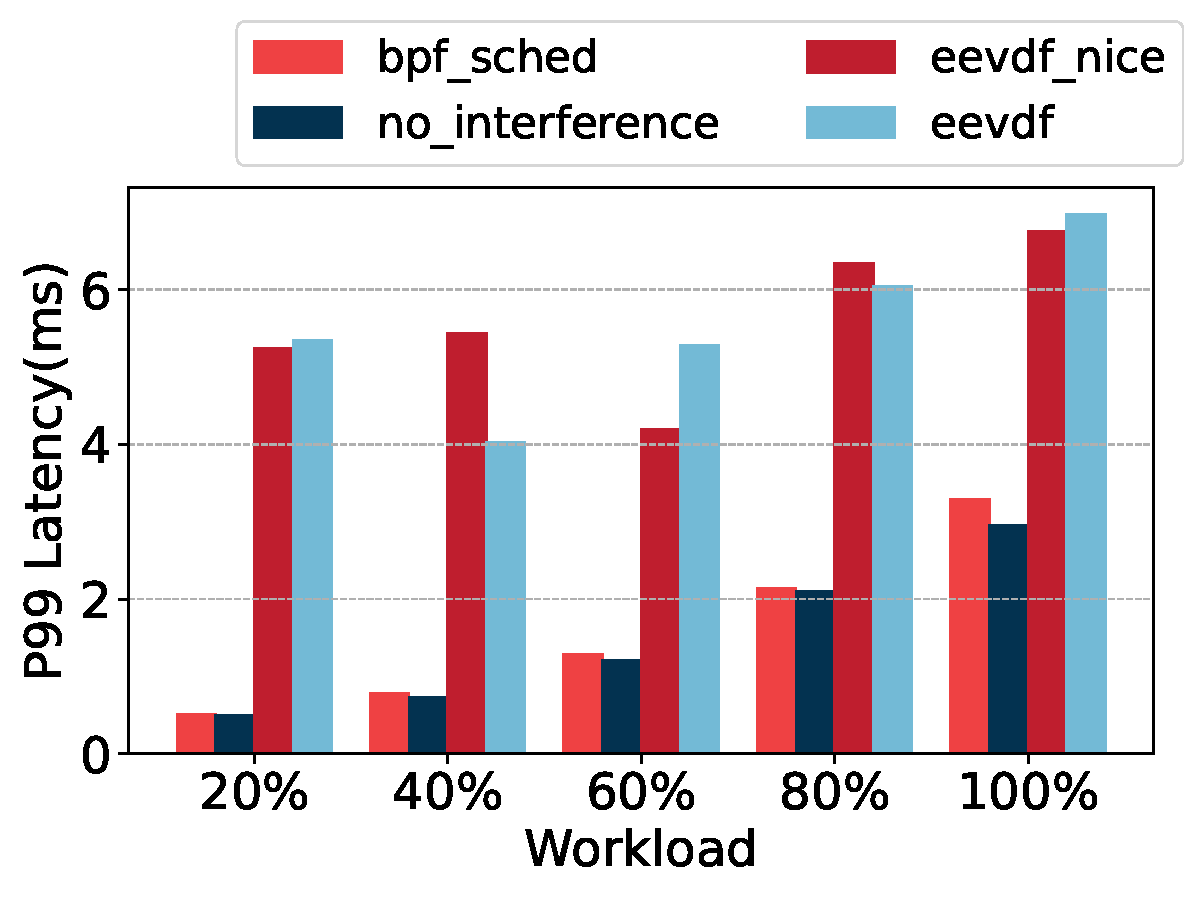
\includegraphics[width=\textwidth]{bpf_sched_smp_redis}
        \bicaption{\quad Redis与干扰混部}{\quad Redis with Interference} 
        \label{fig:bpf_sched_smp_memcached}
    \end{subfigure}
    \begin{subfigure}[b]{0.49\textwidth}
        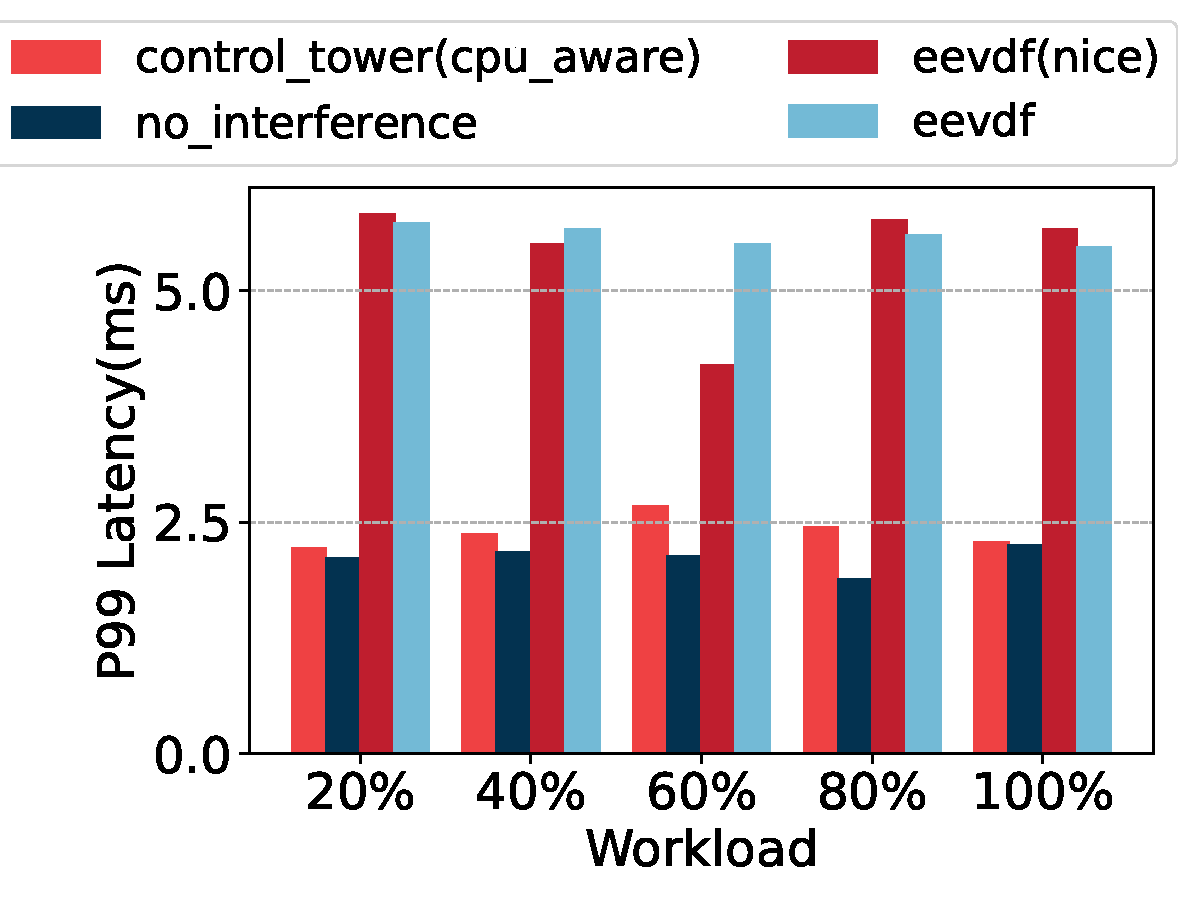
\includegraphics[width=\textwidth]{bpf_sched_smp_memcached}
        \bicaption{\quad Memcached与干扰混部}{\quad Memcached with Interference} 
        \label{fig:bpf_sched_smp_memcached}
    \end{subfigure}
    \begin{subfigure}[b]{0.49\textwidth}
        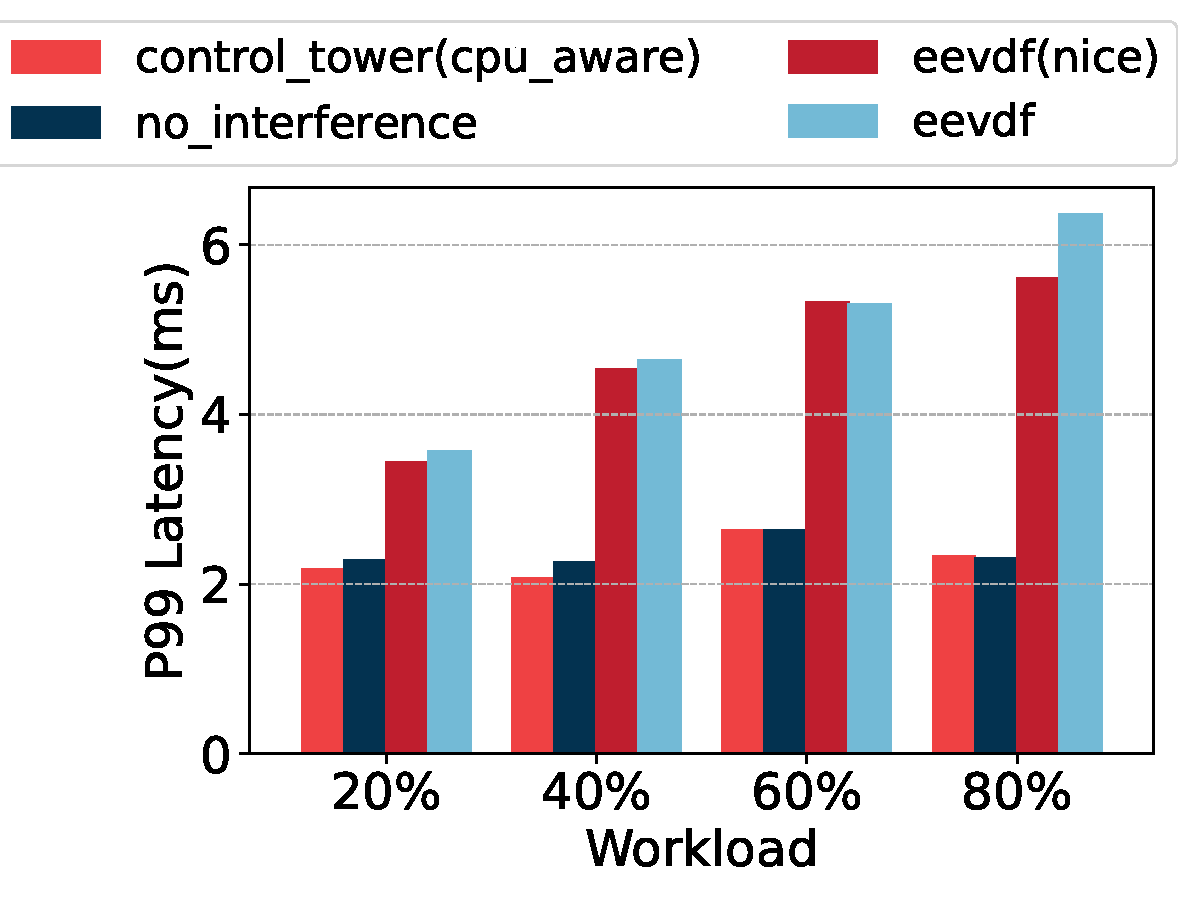
\includegraphics[width=\textwidth]{bpf_sched_smp_nginx}
        \bicaption{\quad Nginx与干扰混部}{\quad Nginx with Interference} 
        \label{fig:bpf_sched_smp_memcached}
    \end{subfigure}
    \begin{subfigure}[b]{0.49\textwidth}
        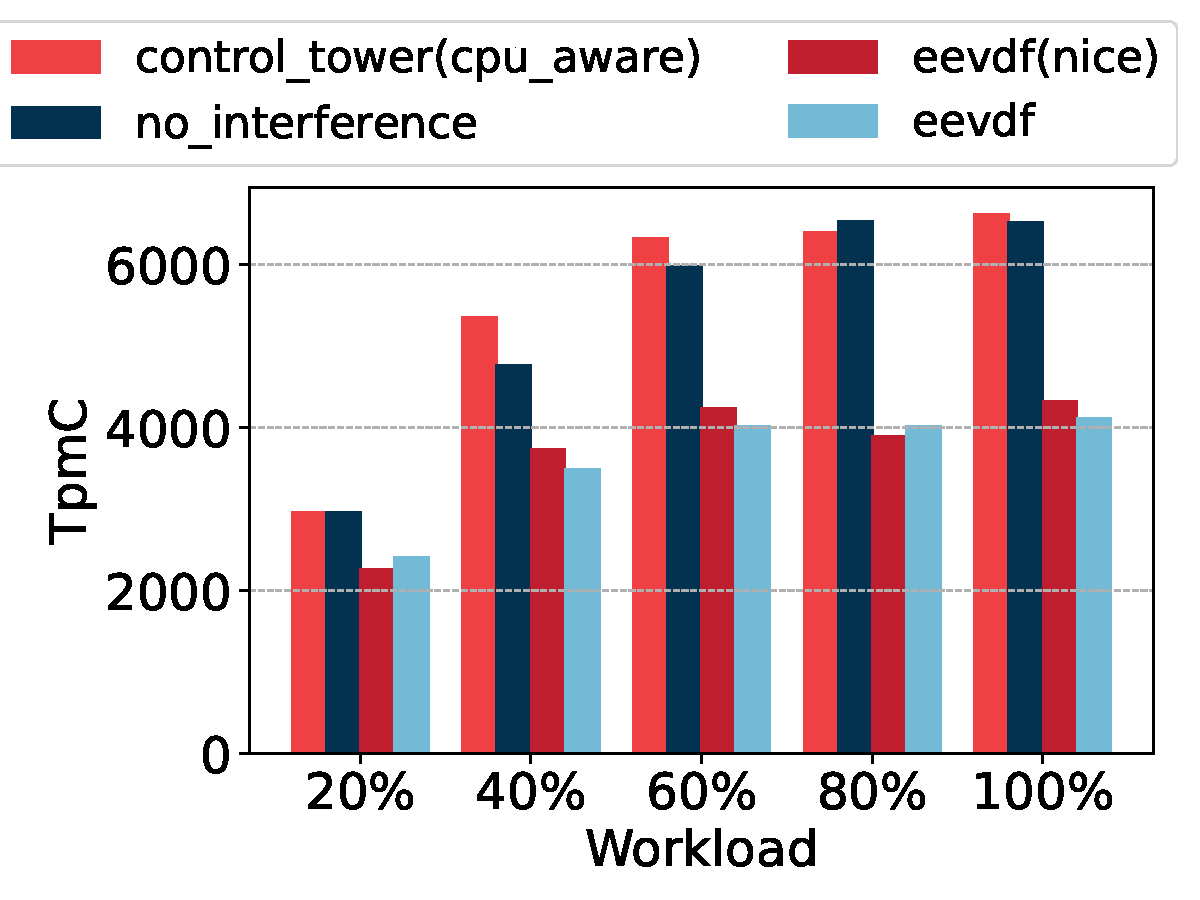
\includegraphics[width=\textwidth]{bpf_sched_smp_mysql}
        \bicaption{\quad Mysql与干扰混部(TpmC)}{\quad MySQL with Interference(TpmC)} 
        \label{fig:bpf_sched_smp_mysql}
    \end{subfigure}
    \begin{subfigure}[b]{0.49\textwidth}
        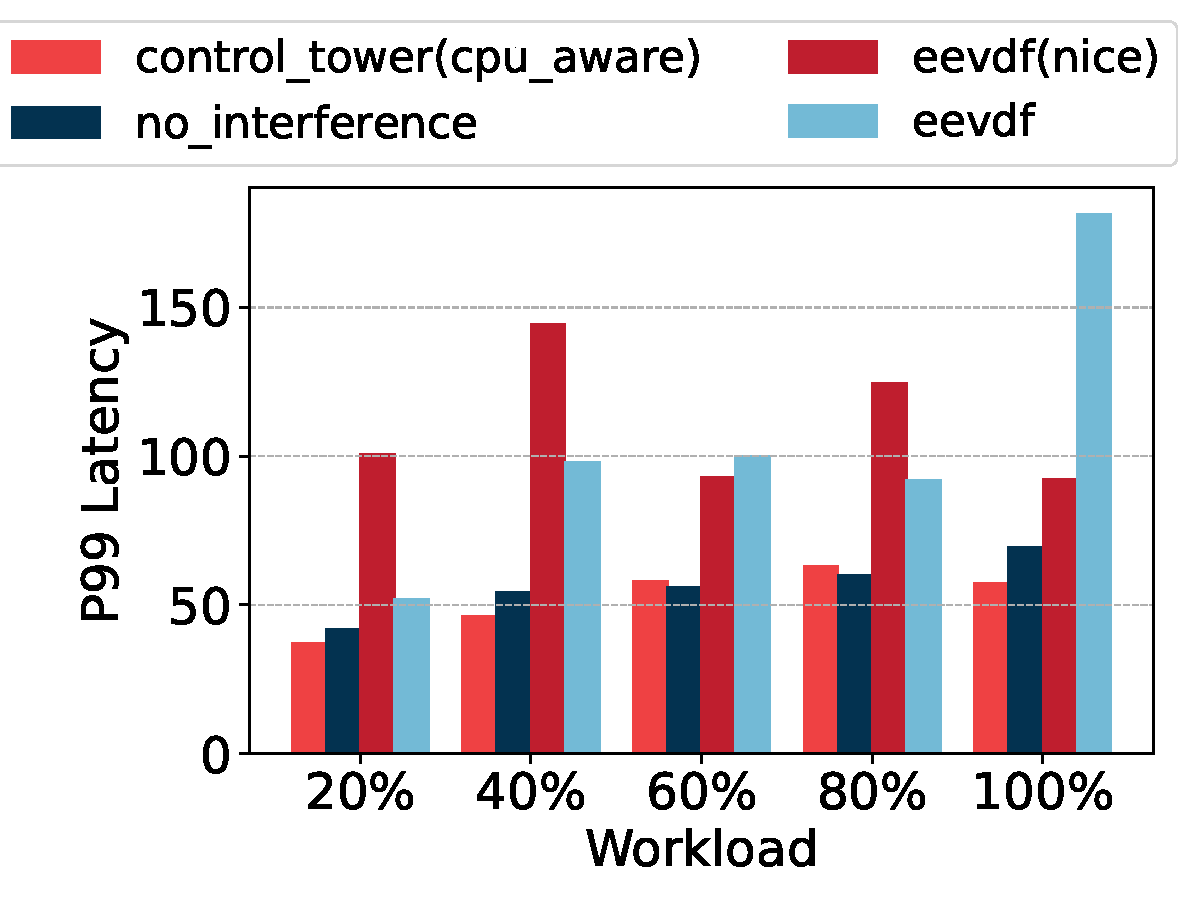
\includegraphics[width=\textwidth]{bpf_sched_smp_mysql_latency}
        \bicaption{\quad Mysql与干扰混部(Latency)}{\quad MySQL with Interference(Latency)} 
        \label{fig:bpf_sched_smp_mysql_latency}
    \end{subfigure}

\bicaption{\quad CPU感知调度下的LC应用QoS保障}{\quad LC Application Latency Stability}
\label{fig:lc_bpf_sched}
\end{figure}

对于SMT场景,由于兄弟核心之间存在片上共享资源,CPU资源感知调度对于这一场景下的QoS保障更为重要,实验在一个2 CPU、1024MB内存的虚拟机中展开,其中CPU配置为兄弟核,同时内核不关闭Core调度机制。实验结果如图~\ref{fig:redis_smt}所示,相较于EEVDF调度器,CPU资源感知BPF调度器在SMT场景中, 能够将Redis延迟最高降低79.6\%,并且最低也有33.7\%的延迟降低效果,同时从图~\ref{fig:lc_box}中能够看出,在CPU资源感知BPF调度器下,Redis的延迟稳定性也得到了一定的保障,这主要是因为CPU资源感知BPF调度器完全运行在内核态中,能够快速的决策并调度任务,从而避免了许多用户态调度器存在的“乒乓效应”。

\begin{figure}[H]
    \centering
    \begin{subfigure}[b]{0.49\textwidth}
        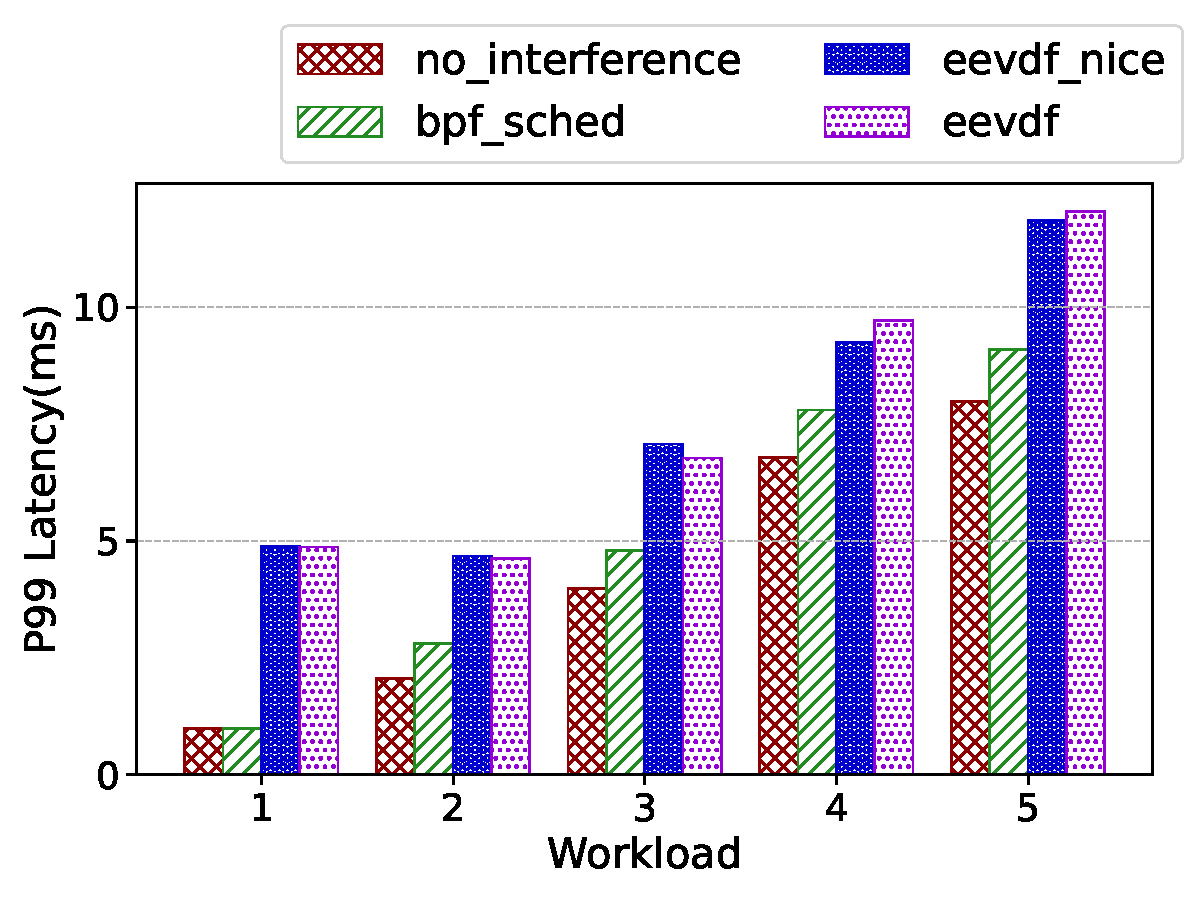
\includegraphics[width=\textwidth]{bpf_sched_smt_redis}
        \bicaption{\quad SMT下Redis与干扰混部}{\quad Redis with Interference On SMT} 
        \label{fig:bpf_sched_smt_redis}
    \end{subfigure}
    \begin{subfigure}[b]{0.49\textwidth}
        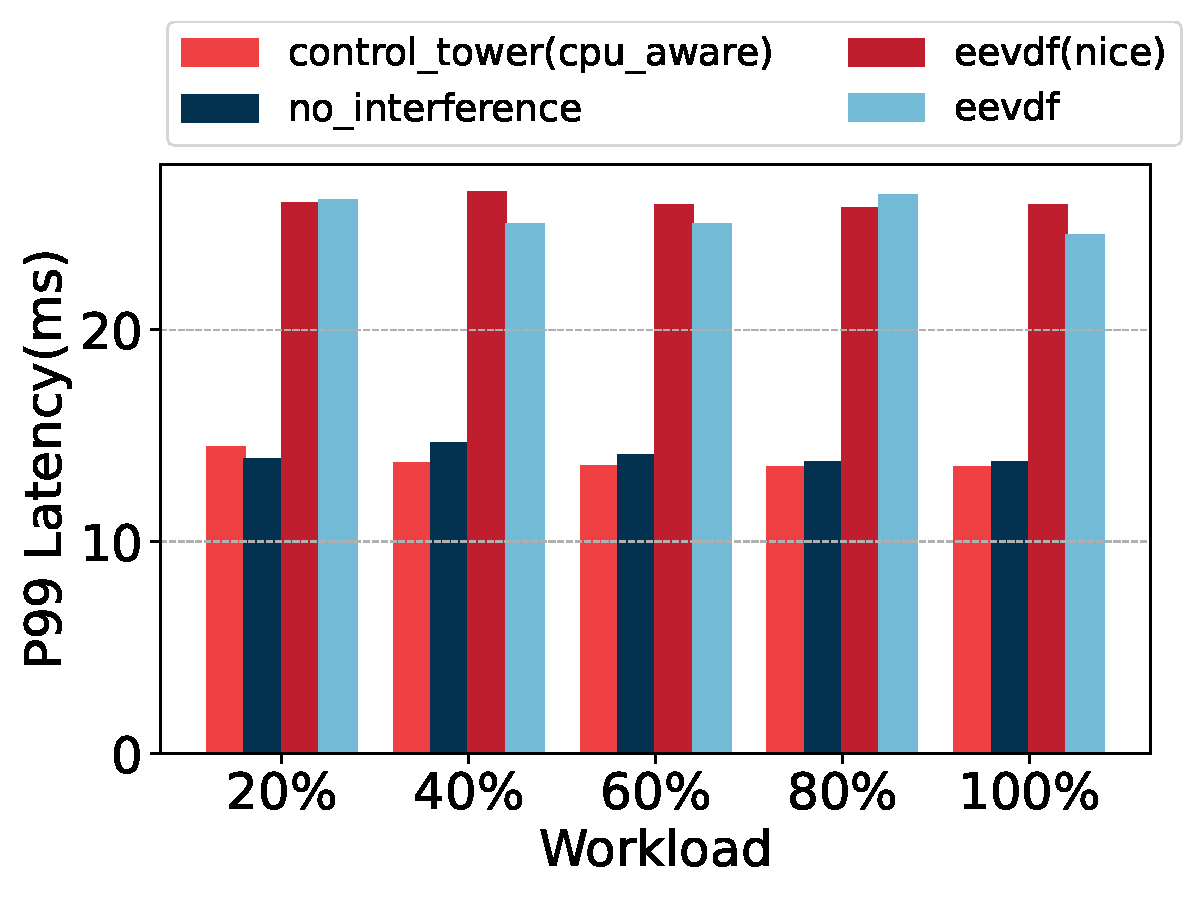
\includegraphics[width=\textwidth]{bpf_sched_smt_memcached}
        \bicaption{\quad SMT下Memcached与干扰混部}{\quad Memcached with Interference On SMT} 
        \label{fig:bpf_sched_smt_memcached}
    \end{subfigure}
    \begin{subfigure}[b]{0.49\textwidth}
        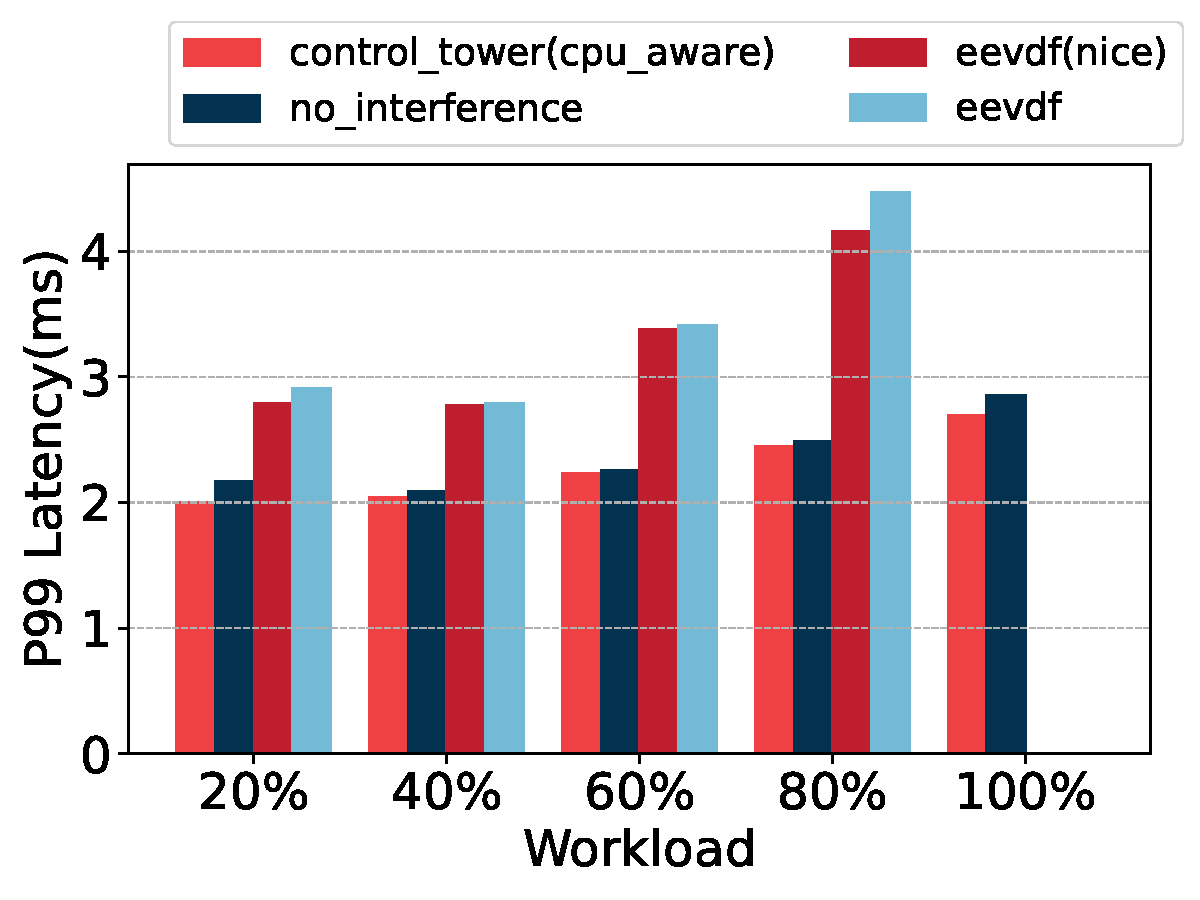
\includegraphics[width=\textwidth]{bpf_sched_smt_nginx}
        \bicaption{\quad SMT下Nginx与干扰混部}{\quad Nginx with Interference On SMT} 
        \label{fig:bpf_sched_smt_nginx}
    \end{subfigure}
    \begin{subfigure}[b]{0.49\textwidth}
        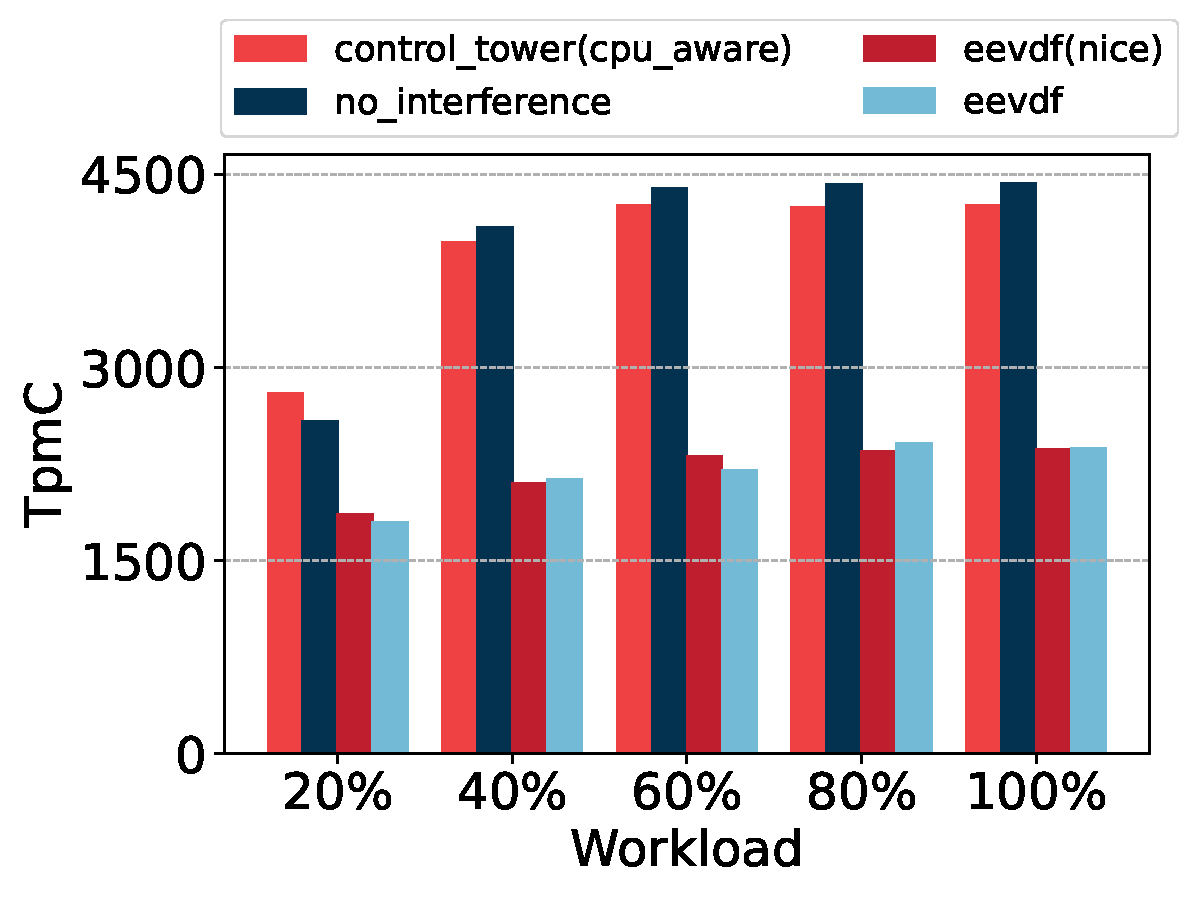
\includegraphics[width=\textwidth]{bpf_sched_smt_mysql}
        \bicaption{\quad SMT下Mysql与干扰混部(TpmC)}{\quad Mysql with Interference On SMT(TpmC)} 
        \label{fig:bpf_sched_smt_mysql}
    \end{subfigure}
    \begin{subfigure}[b]{0.49\textwidth}
        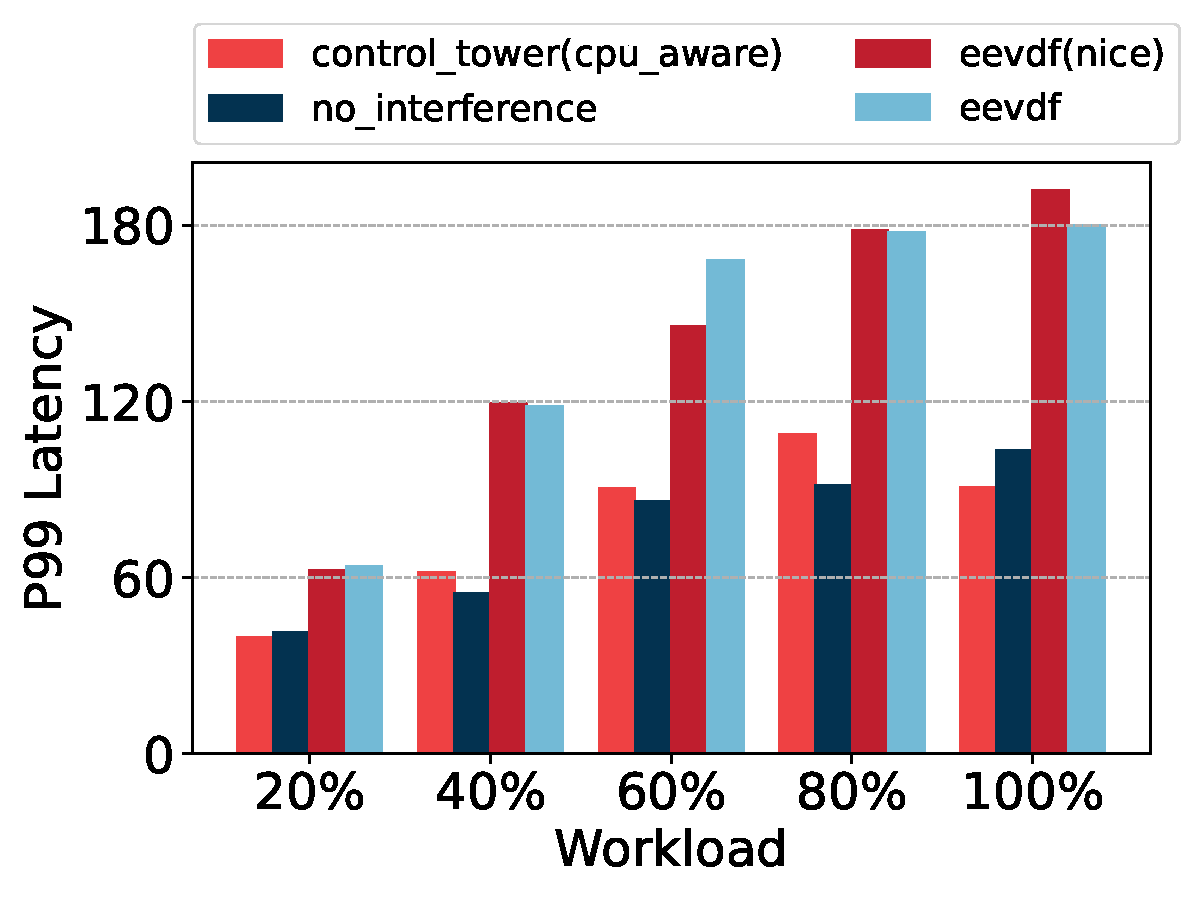
\includegraphics[width=\textwidth]{bpf_sched_smt_mysql_latency}
        \bicaption{\quad SMT下Mysql与干扰混部(Latency}{\quad Mysql with Interference On SMT(Latency)} 
        \label{fig:bpf_sched_smt_mysql_latency}
    \end{subfigure}
\bicaption{\quad CPU感知调度下的LC应用QoS保障}{\quad LC Application Latency Stability}
\label{fig:lc_bpf_sched}
\end{figure}

\begin{figure}[H]
    \centering
    \begin{subfigure}[b]{0.4\textwidth}
        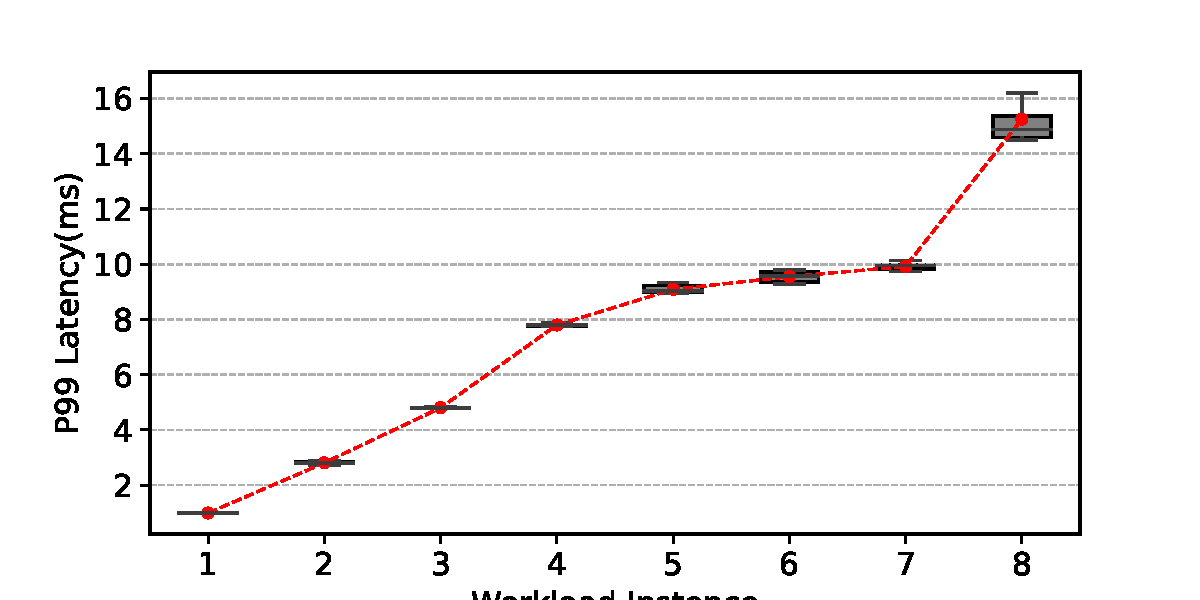
\includegraphics[width=\textwidth]{cpu_aware_box_bpf_sched}
        \caption{无干扰下Redis延迟}
        \label{fig:cpu_aware_box_bpf_sched}
    \end{subfigure}
    \begin{subfigure}[b]{0.4\textwidth}
        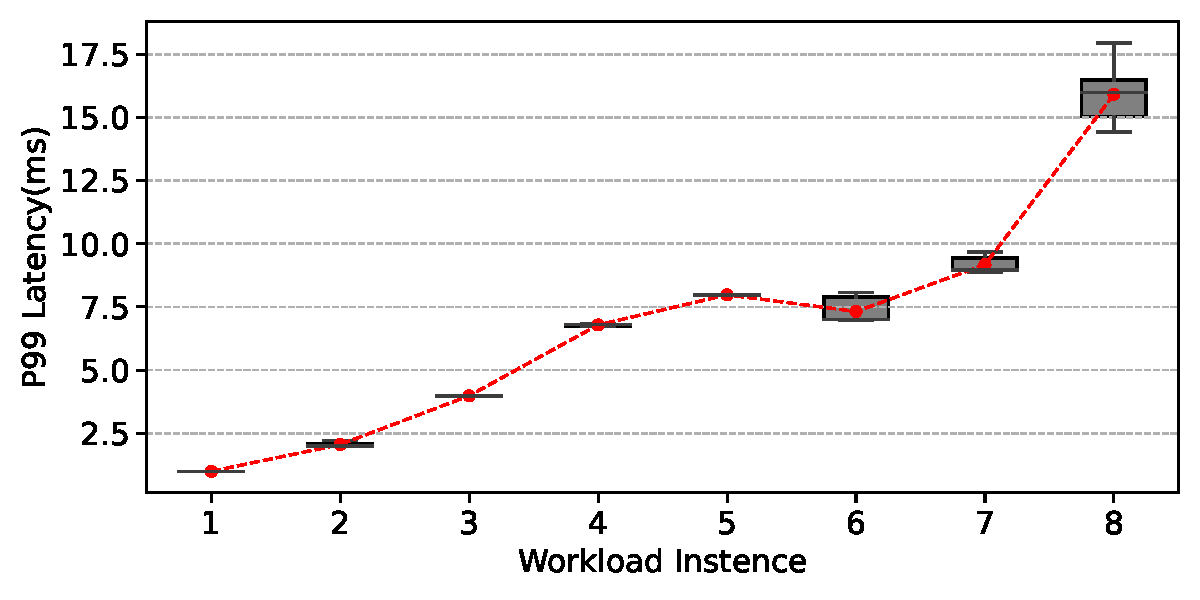
\includegraphics[width=\textwidth]{cpu_aware_box_no_interference}
        \caption{混部场景BPF调度器}
        \label{fig:cpu_aware_box_no_interference}
    \end{subfigure}
    \begin{subfigure}[b]{0.4\textwidth}
        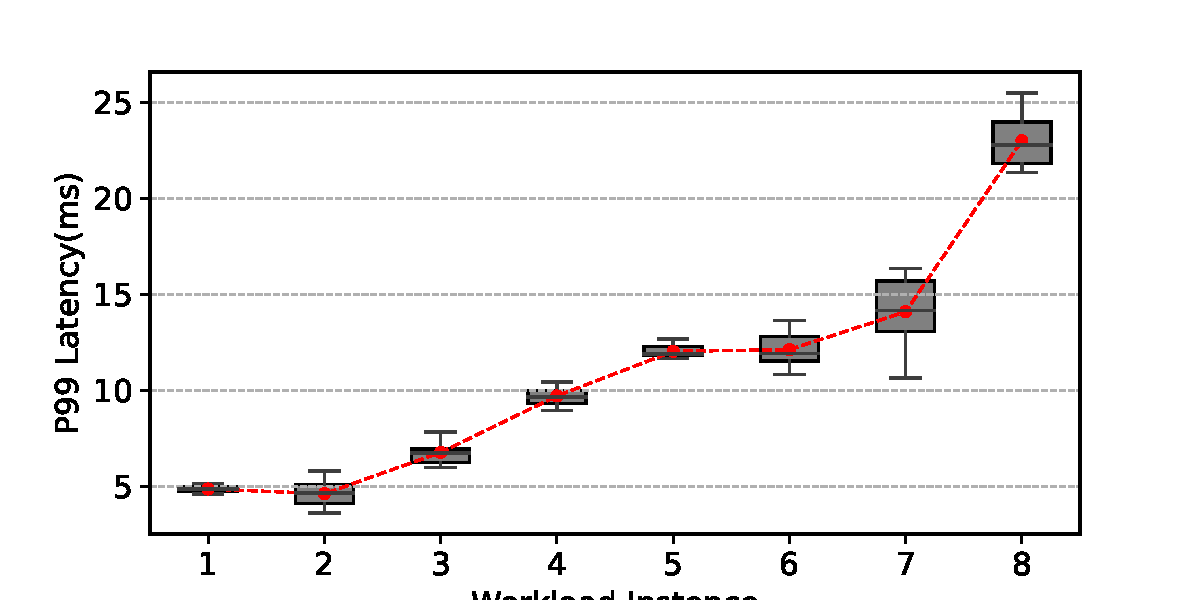
\includegraphics[width=\textwidth]{cpu_aware_box_eevdf}
        \caption{混部场景EEVDF调度器}
        \label{fig:cpu_aware_box_eevdf}
    \end{subfigure}
    \begin{subfigure}[b]{0.4\textwidth}
        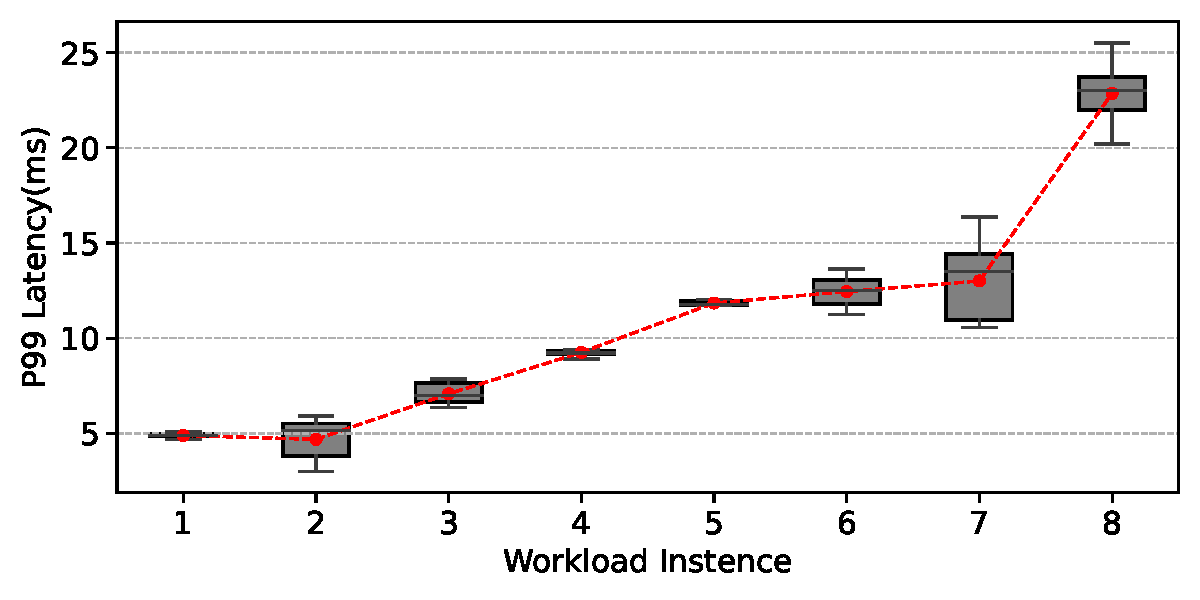
\includegraphics[width=\textwidth]{cpu_aware_box_eevdf_nice}
        \caption{混部场景EEVDF高优先级}
        \label{fig:cpu_aware_box_eevdf_nice}
    \end{subfigure}
\bicaption{\quad LC应用延迟稳定性}{\quad LC Application Latency Stability}
\label{fig:lc_box}
\end{figure}

% \subsection{网络资源感知策略}

% \subsection{内存资源感知策略}
% Redis

\section{本章小结}

本章主要首先针对画像分析中不同类型应用,基于内核中关于HZ与抢占模型的配置,设计了调度配置的定制优化,提供了吞吐量优先与响应度优先两种不同调度目标的内核配置。

随后设计了混部场景下高优先应用与低优先级应用基于BPF调度策略的QoS保障机制,首先,提出了较为粗粒度的BPF调度队列隔离策略,利用调度类的优先级特性,使得在单个CPU上,低优先级能够感知高优先级任务的执行并出让CPU资源,从而保障高优先级应用的执行。

其次,基于BPF调度队列隔离策略,结合eBPF对于CPU与网络资源的感知实现更灵活的BPF资源感知调度策略,一方面相较于静态的CPU亲和性配置,CPU资源感知的调度策略能够动态地利用高优先级任务没有用到的核心,另一方面利用eBPF程序之间的交互性,能够方便地将其他子系统中的监测信息传递给BPF Scheduler进行辅助决策。

最后,比较了不同内核下的应用性能,说明对于不同的应用而言,定制的内核能够在一定程度上提升其运行性能。最后,通过不同应用,不同硬件环境下的混部实验,说明了使用BPF Scheduler来针对不同的混部场景进行定制优化,在提升高优先级应用的性能保障效果上的优势。